\documentclass[]{beamer}
\usepackage[utf8]{inputenc}
\usepackage[T1]{fontenc}
\usepackage{carlito}
\usetheme[horizontal=true, hr=false, pagenumbers=true]{NewPwr}
\usepackage{bibentry}
\usepackage{minted}
\setminted{fontsize=\small,baselinestretch=1}
\usepackage{multicol}
\usepackage{polski}
\usepackage{setspace}

% Build-specific command
\nonstopmode

%Information to be included in the title page:
\title{Opracowanie algorytmu generacji grafu DSP do rozwiązania problemu syntezy dźwięku}
\subtitle{Design of a DSP graph generation algorithm for solving the sound synthesis problem}
\author{Autor pracy: Mateusz Bączek \\ Opiekun pracy: Dr Inż. Maciej Hojda}
% \institute{Seminarium Dyplomowe -- prezentacja 1}
\date{2023}

\begin{document}
\onehalfspacing
\frame{\titlepage}

\section{Wstęp teoretyczny}


\begin{frame}
  \frametitle{Sztuka generatywna, algorytmiczna kompozycja muzyki}

  \begin{multicols}{2}

  \begin{figure}
    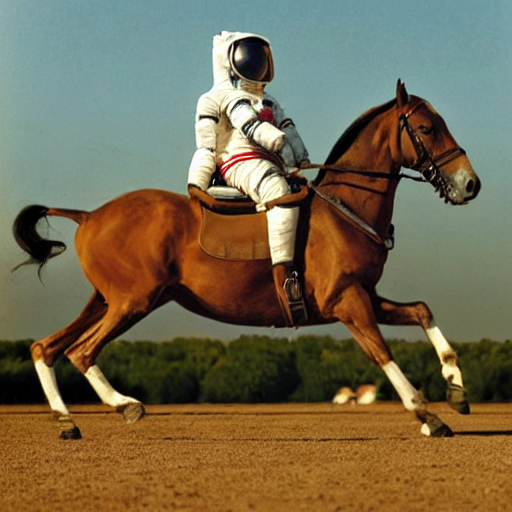
\includegraphics[width=0.9\linewidth]{stable_diffusion.png}
    \caption{Obraz wygenerowany za pomocą algorytmu \textit{Stable Diffusion}.}
  \end{figure}

  \begin{figure}
    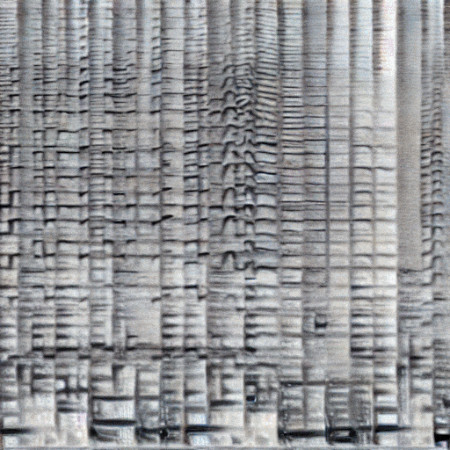
\includegraphics[width=0.8\linewidth]{riffusion_spectro.jpg}
    \caption{Spektrogram wygenerowany za pomocą algorytmu \textit{Stable Riffusion}.}
  \end{figure}

  \end{multicols}
\end{frame}

\begin{frame}
  \frametitle{Popularne podejścia do kompozycji algorytmicznej}

  \begin{enumerate}
    \item Generowanie zapisu nutowego \cite{language_models_drummers},
      % \begin{itemize}
      %   \item wykorzystuje reguły matematyczne oparte o teorię muzyki,
      %   \item generuje zapis symboliczny, który łatwo później wykorzystać.
      % \end{itemize}
    \item Generowanie pełnego pliku audio \cite{riffusion},
      % \begin{itemize}
      %   \item teoretycznie najbardziej imponujący efekt działania,
      %   \item małe możliwości wykorzystania rezultatu algorytmu.
      % \end{itemize}
    \item Symulacja instrumentów za pomocą sieci neuronowych \cite{nsynth}.
      % \begin{itemize}
      %   \item potencjalnie bardzo szeroka gama generowanych brzmień,
      %   \item małe możliwości dostosowania brzmienia,
      %   \item słaby wgląd we ,,wnętrze'' wygenerowanego algorytmu DSP.
      % \end{itemize}
  \end{enumerate}
\end{frame}

% \begin{frame}
%   \frametitle{Elementy kompozycji muzycznej (w uproszczeniu)}
%   \begin{figure}[H]
%     \centering\small
%     \begin{center}
%     \begin{tikzpicture}
%       \begin{scope}[blend group = soft light]
%         \fill[red!30!white]    ( 90:1.5) circle (1.7);
%         \fill[blue!30!white]   (210:1.5) circle (1.7);
%         \fill[orange!30!white] (330:1.5) circle (1.7);
%       \end{scope}
%       \node at (90: 1.5) [align=center] {\small Linia \\ melodyczna};
%       \node at (210:1.5) [align=center] {\small Modulacja};
%       \node at (330:1.5) [align=center] {\small Barwa \\ dźwięku};
%       % \node[align=center] { \textbf{Wspólna} \\ \textbf{pętla zdarzeń} \\ \textbf{\texttt{asyncio}}};
%     \end{tikzpicture}
%     \end{center}
%     \caption{
%       Elementy opisujące pojedynczy głos/instrument w kompozycji muzycznej. 
%     }
%     \label{telemetry_backend_asyncio}
%   \end{figure}
% \end{frame}


\section{Opis i cel pracy}
\begin{frame}
  \frametitle{Cel pracy}

  \centering
  \Large
    Wytworzenie grafu przetwarzania sygnałów, który geneneruje dźwięk o określonej \colorbox{blue}{\color{white}\textbf{barwie}}.

  % \vspace{0.5cm}

  % \begin{multicols}{2}
    \begin{figure}
      \centering
      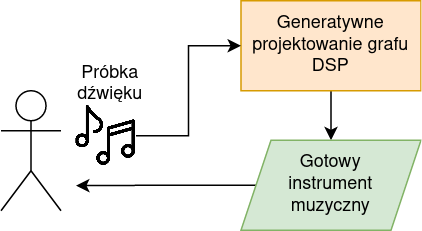
\includegraphics[width=0.4\linewidth]{use_case_diagram.png}
      \caption{Ilustracja przypadku użycia.}
    \end{figure}

    % \begin{figure}
    %   \centering
    %   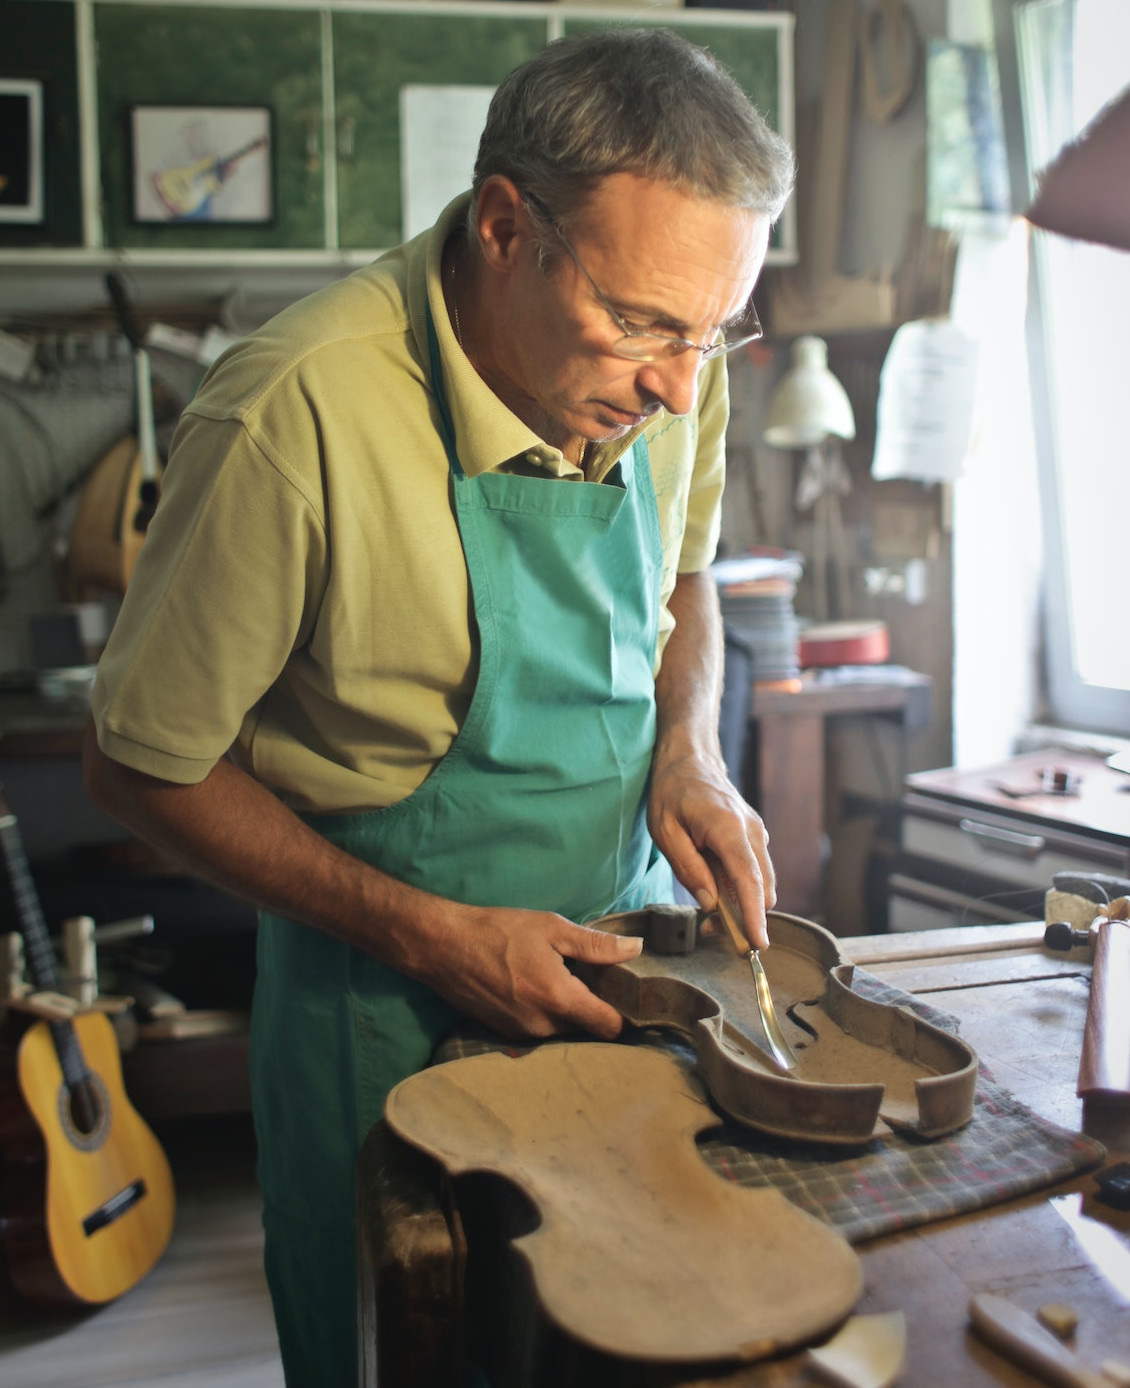
\includegraphics[width=0.6\linewidth]{luthier_person.jpg}
    %   \caption{Lutmistrz przy pracy.}
    % \end{figure}
  % \end{multicols}
\end{frame}


\begin{frame}
  \frametitle{Czym jest \textbf{barwa} dźwięku?}
  \begin{figure}
    \centering
    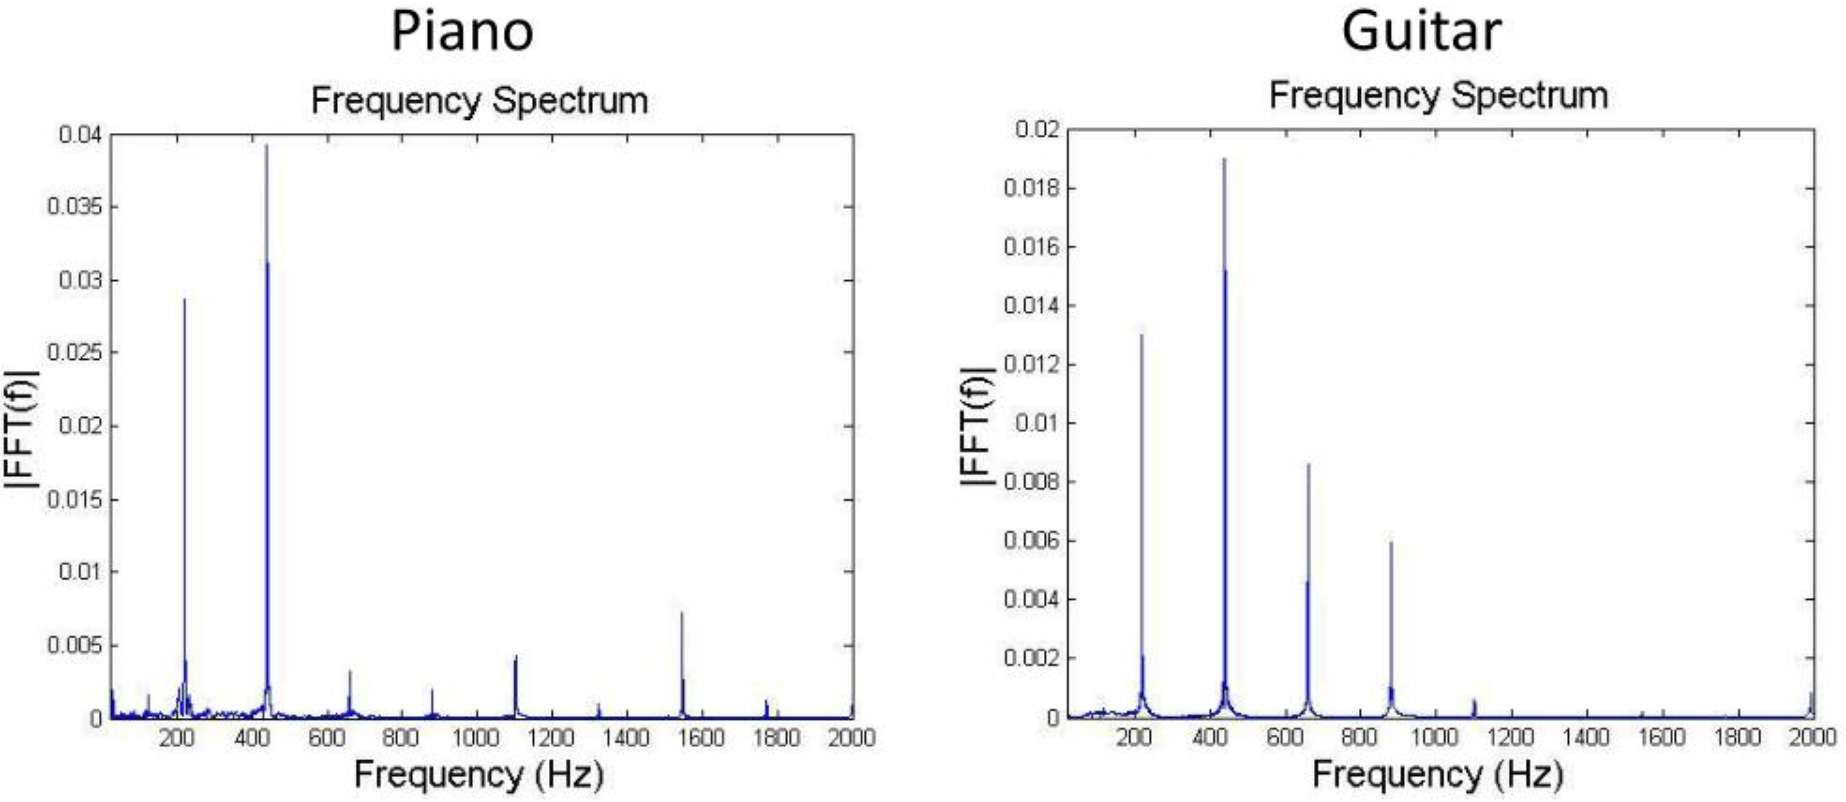
\includegraphics[width=0.9\linewidth]{piano_guitar_fourier.png}
    \caption{Porównanie transformaty Fouriera dla tej samej nuty granej na pianinie i na gitarze.}
  \end{figure}
\end{frame}


% \begin{frame}
%   \frametitle{Czym jest \textbf{barwa} dźwięku?}
%   \begin{figure}
%     \centering
%     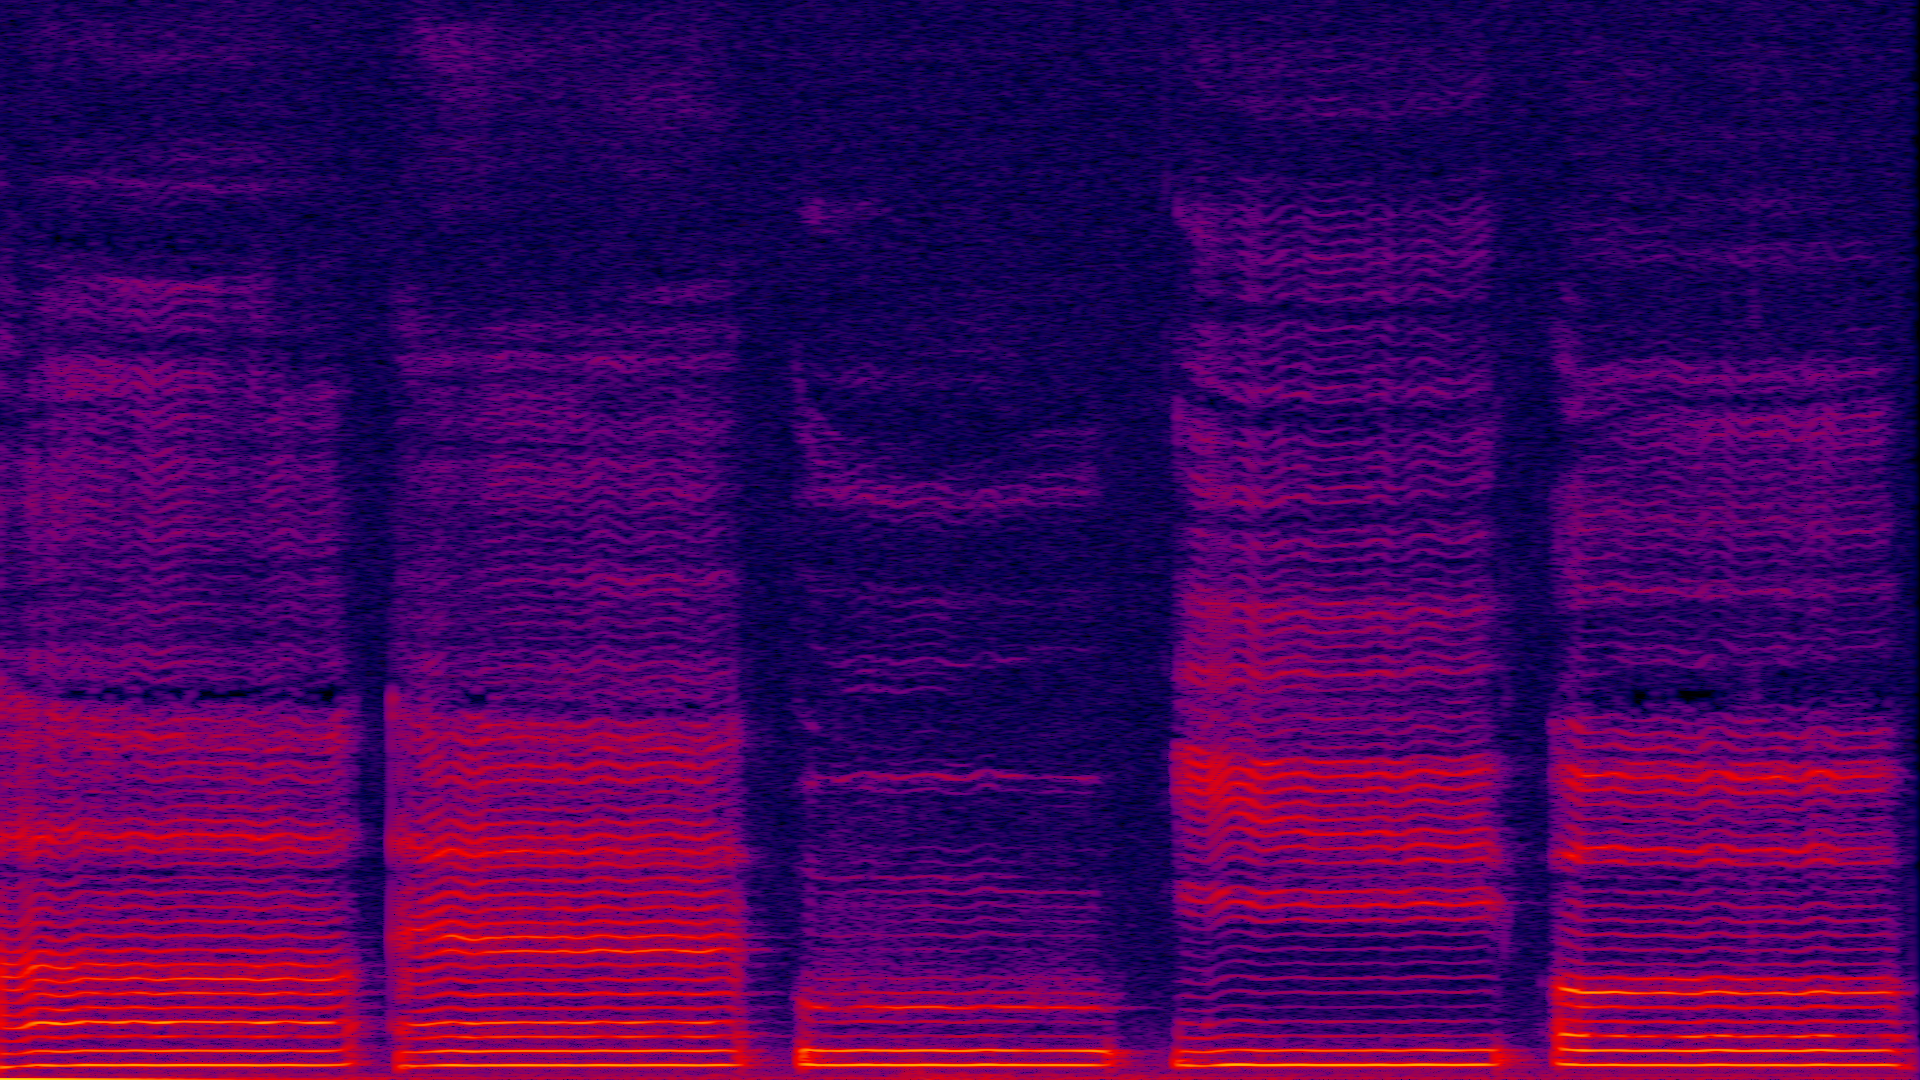
\includegraphics[width=0.9\linewidth]{aeuio_spectrogram.png}
%     \caption{Spektrogram (transformata Fouriera w czasie) dla nagrania samogłosek ,,,a, e, u, i, o''.}
%   \end{figure}
% \end{frame}


\begin{frame}
  \frametitle{Problemy rozwiązywane w ramach pracy}

  \begin{multicols}{2}

  \begin{enumerate}
    \item Jak \textbf{wygenerować} dźwięk?
    \item Jak \textbf{ocenić}, czy dźwięk spełnia zadane wymagania?
    \item Jak \textbf{zmodyfikować} generowany dźwięk, aby zbliżyć się do wymaganego brzmienia?
  \end{enumerate}

  \begin{figure}
    \centering
    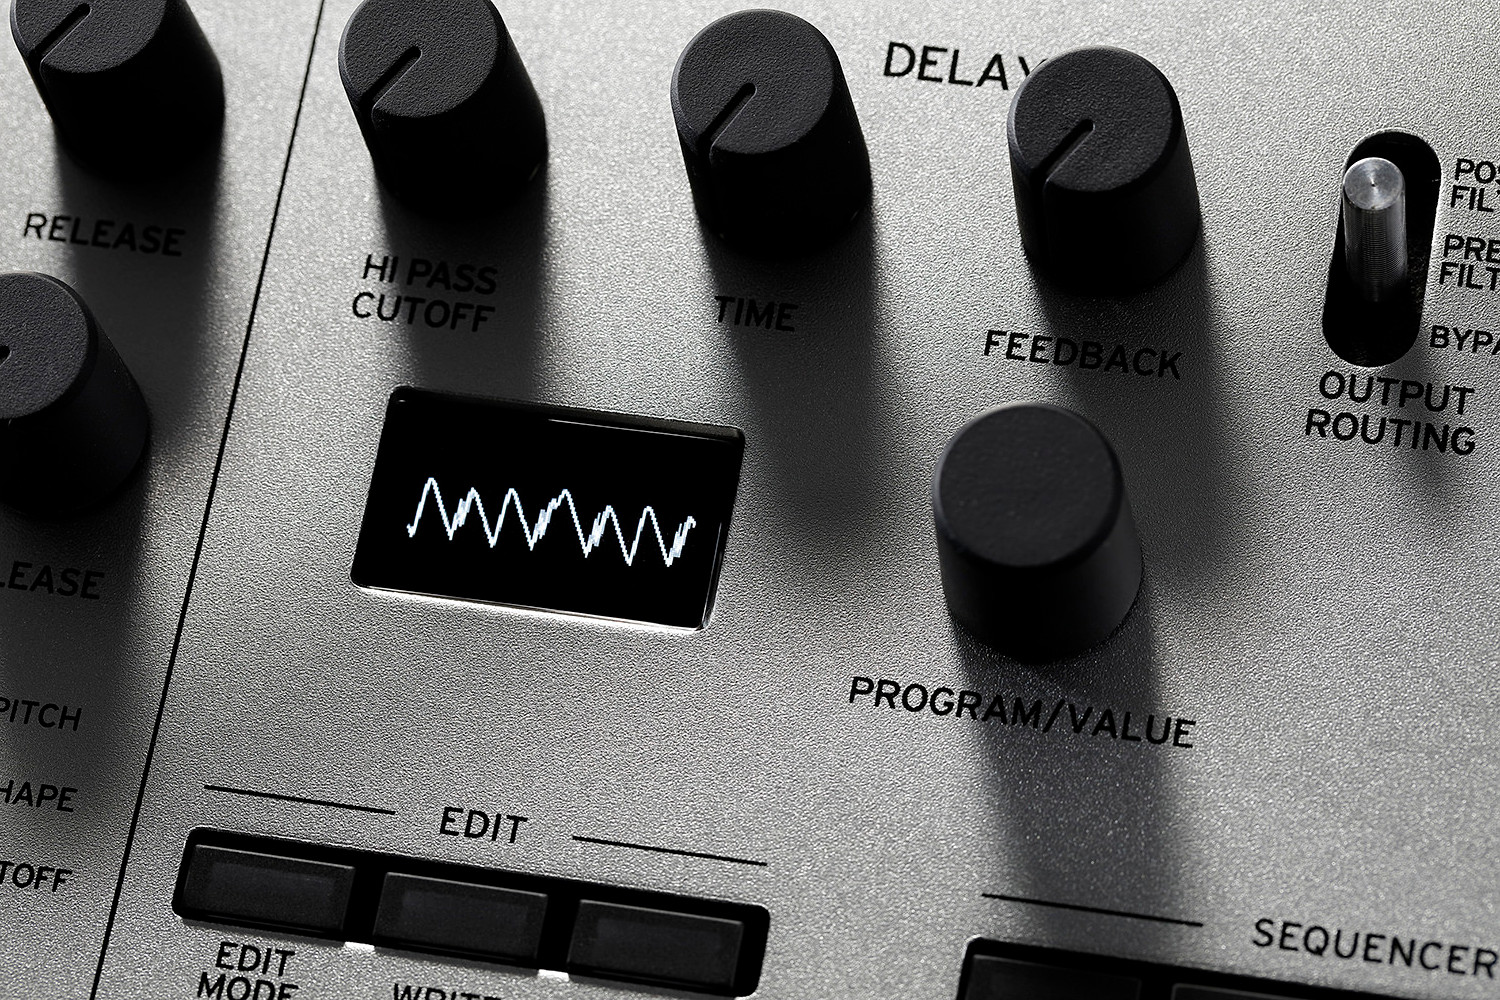
\includegraphics[width=1.0\linewidth]{minilogue_oscillator.jpg}
    \caption{Przebieg sygnału dźwiękowego na oscyloskopie.}
  \end{figure}
  \end{multicols}

\end{frame}

\begin{frame}
  \frametitle{Skąd bierze się barwa dźwięku?}
  \begin{itemize}
    \item Materiał, z którego wykonane są struny,
    \item pudło rezonansowe (lub jego brak),
    \item kształt pudła rezonansowego,
    \item materiał, z którego wykonany jest instrument,
    \item materiał, który uderza w struny,
    \item ... i wiele innych cech fizycznych instrumentu.
  \end{itemize}
\end{frame}

\section{O syntezie dźwięku}

\begin{frame}
  \frametitle{Architektura instrumentu muzycznego}

  \begin{itemize}
    \item Generacja sygnału,
    \item filtracja sygnału,
    \item efekty dźwiękowe.
  \end{itemize}

  \begin{figure}
    \centering
    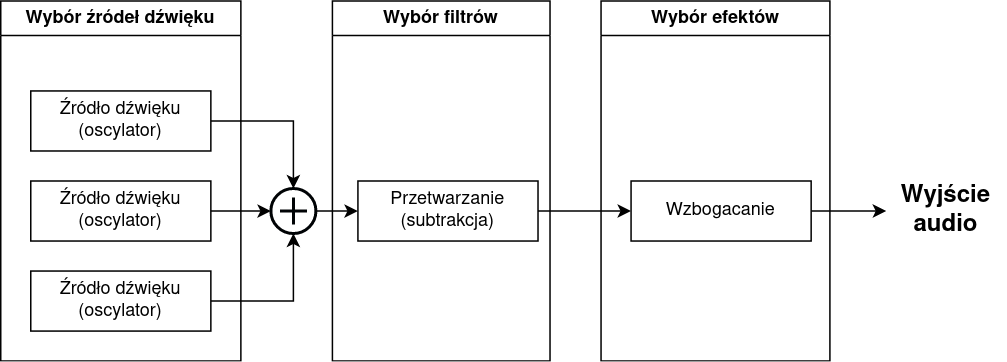
\includegraphics[width=0.7\linewidth]{synth_architecture.png}

    \caption{
      Architektura instrumentu muzycznego.
    }
  \end{figure}
\end{frame}

\begin{frame}
  \frametitle{Jak kontroluje się barwę w syntezatorach dźwięku}

  \begin{figure}
    \centering
    % 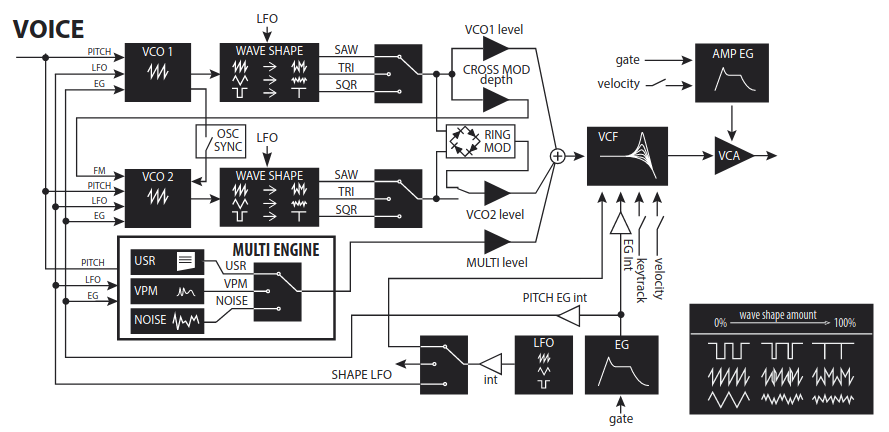
\includegraphics[width=0.9\linewidth]{minilogue_voice_block_diagram.png}
    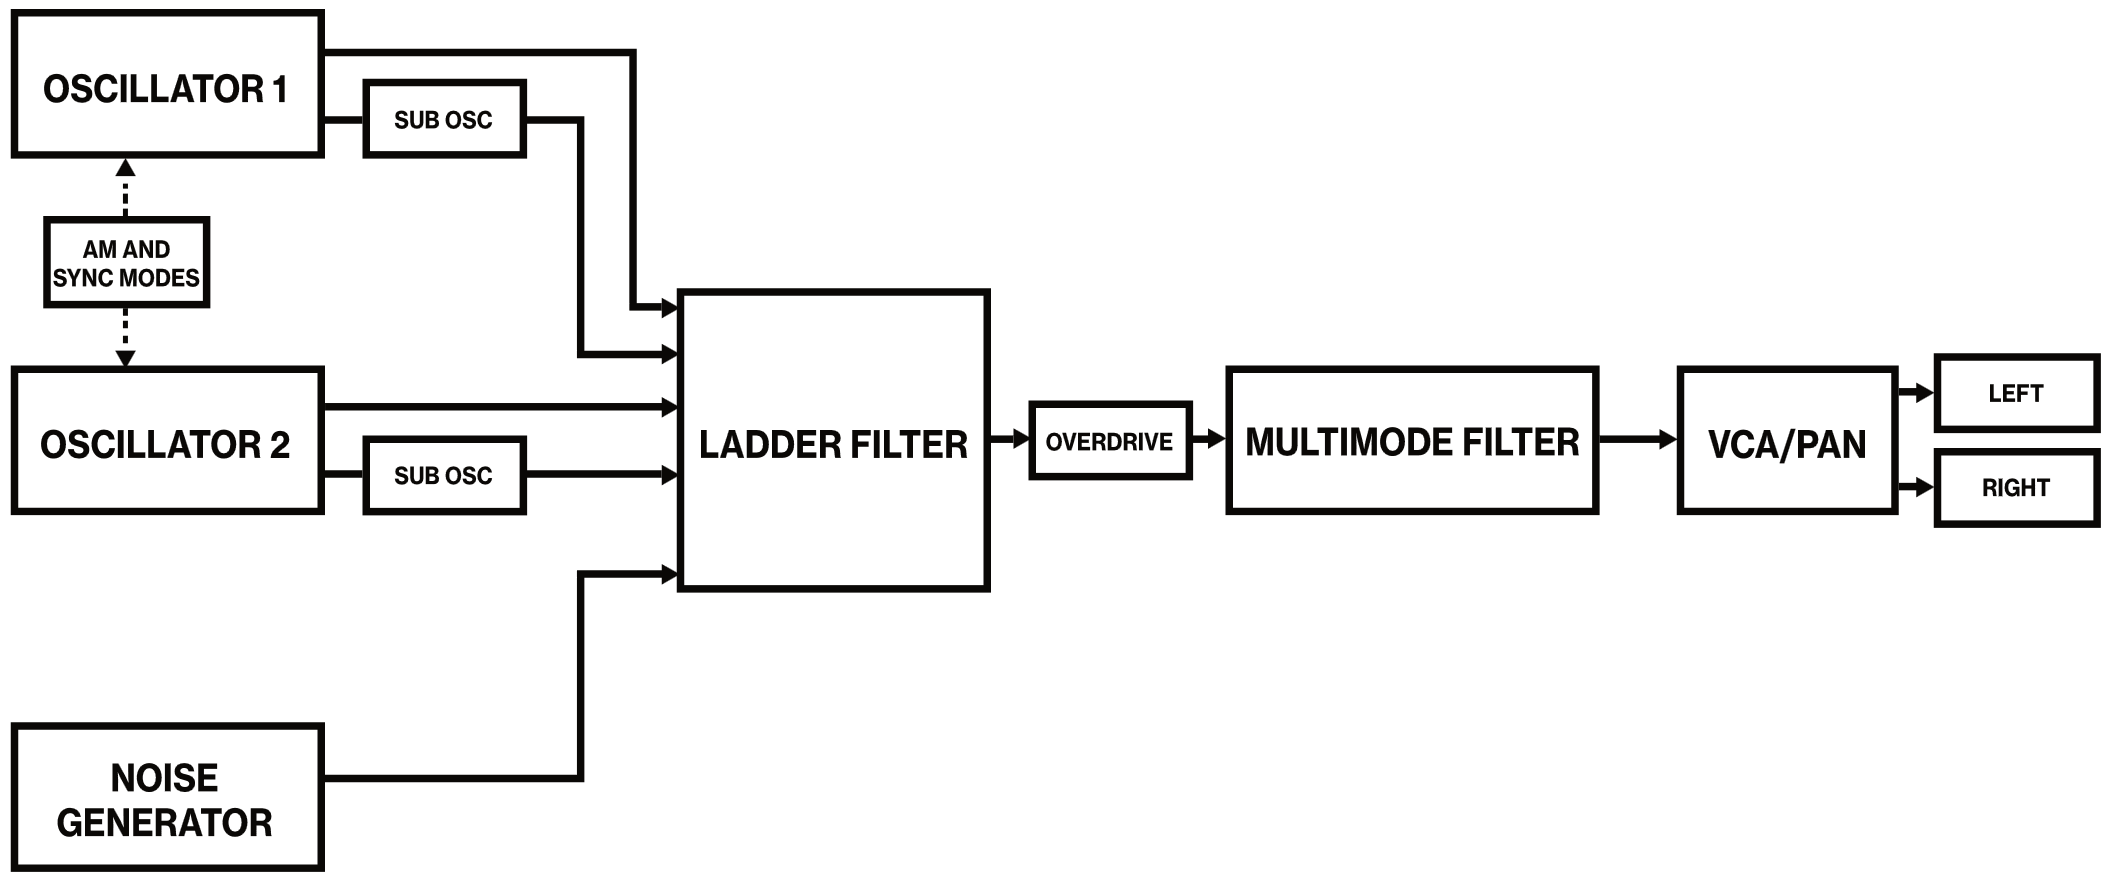
\includegraphics[width=0.9\linewidth]{analog_four_diagram.png}

    \caption{
      Diagram blokowy pojedynczego głosu w syntezatorze 
      \textit{Elektron Analog Four}.
    }
  \end{figure}
\end{frame}

\begin{frame}
  \frametitle{Jak kontroluje się barwę w syntezatorach dźwięku}

  \begin{figure}
    \centering
    % 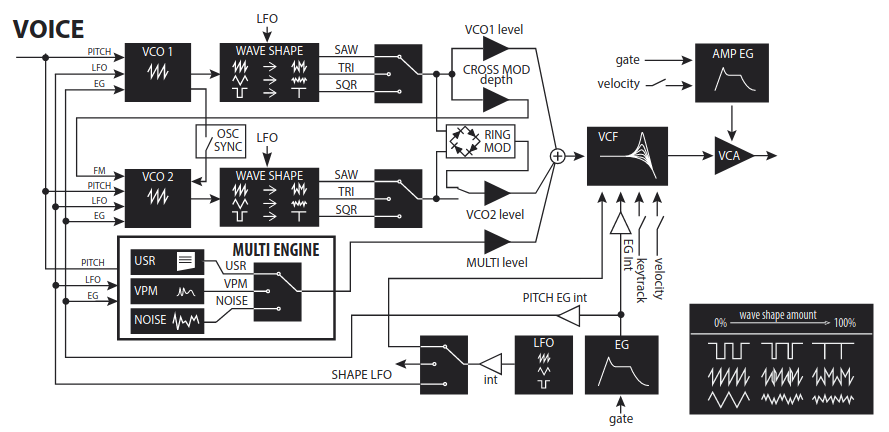
\includegraphics[width=0.9\linewidth]{minilogue_voice_block_diagram.png}
    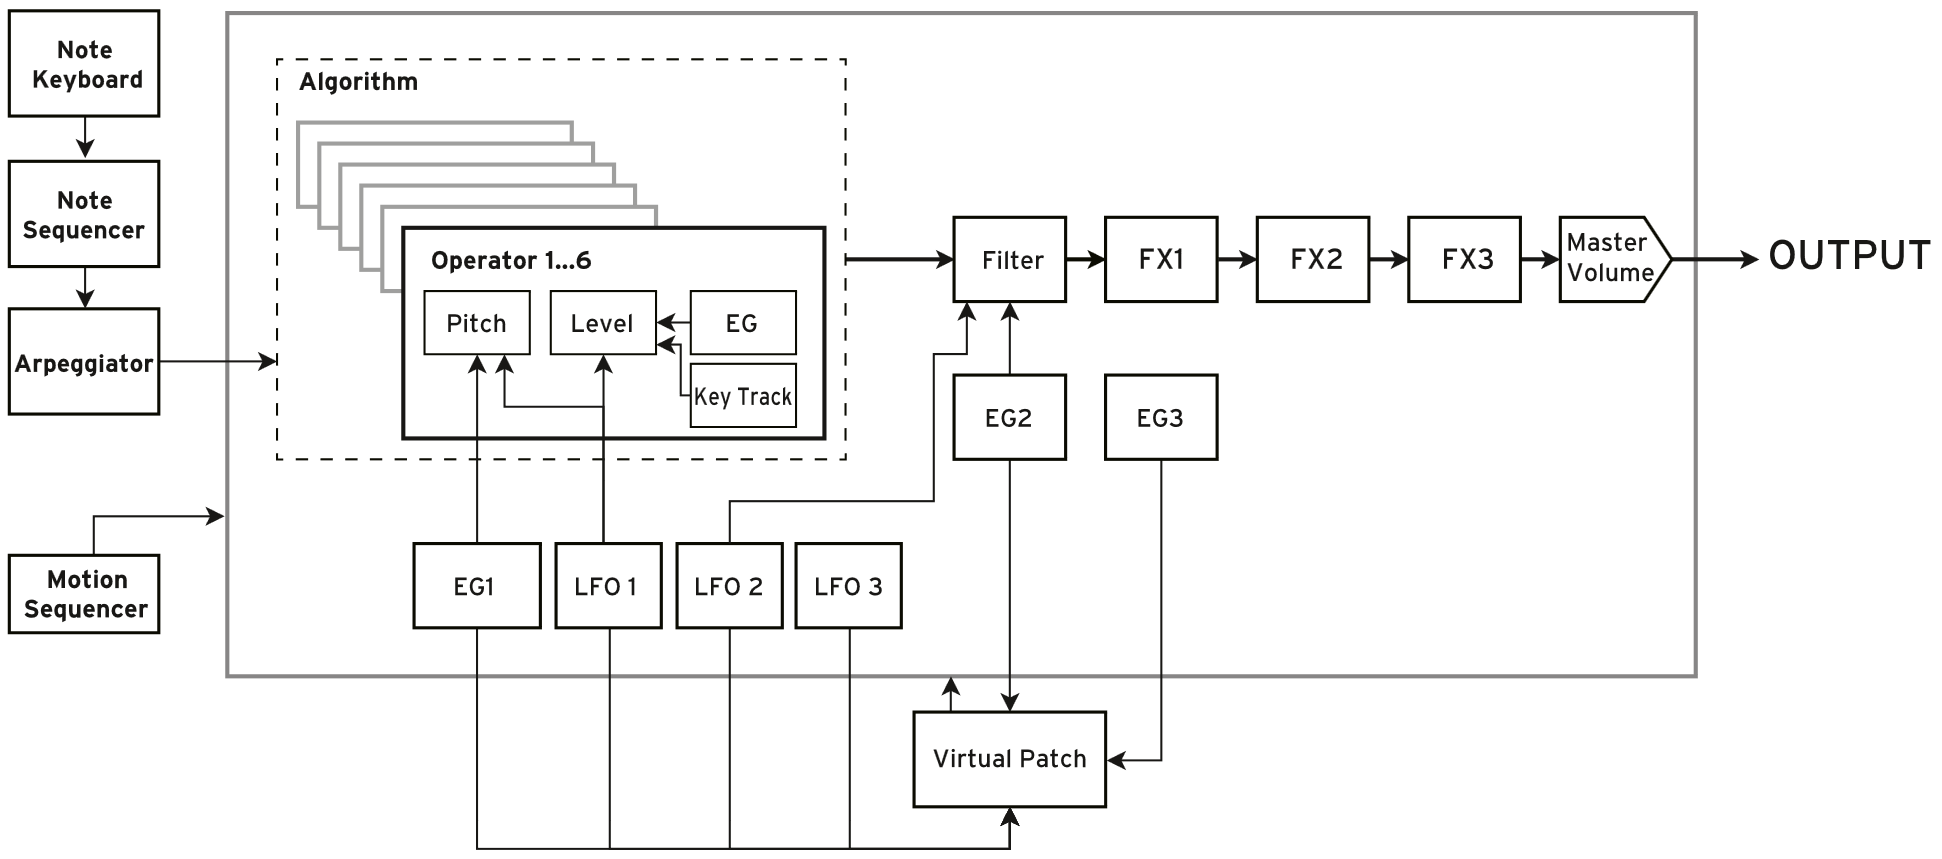
\includegraphics[width=0.9\linewidth]{opsix_diagram.png}

    \caption{
      Diagram blokowy pojedynczego głosu w syntezatorze 
      \textit{Korg Opsix}.
    }
  \end{figure}
\end{frame}

\begin{frame}
  \frametitle{Jak kontroluje się barwę w syntezatorach dźwięku}

  \begin{figure}
    \centering
    % 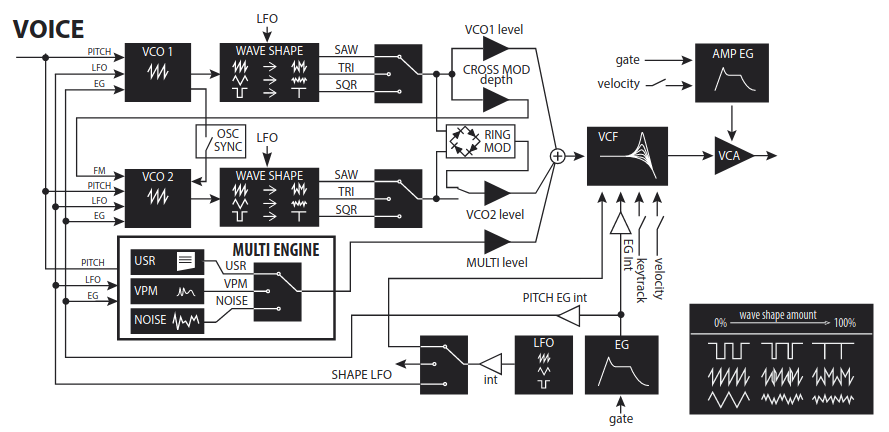
\includegraphics[width=0.9\linewidth]{minilogue_voice_block_diagram.png}
    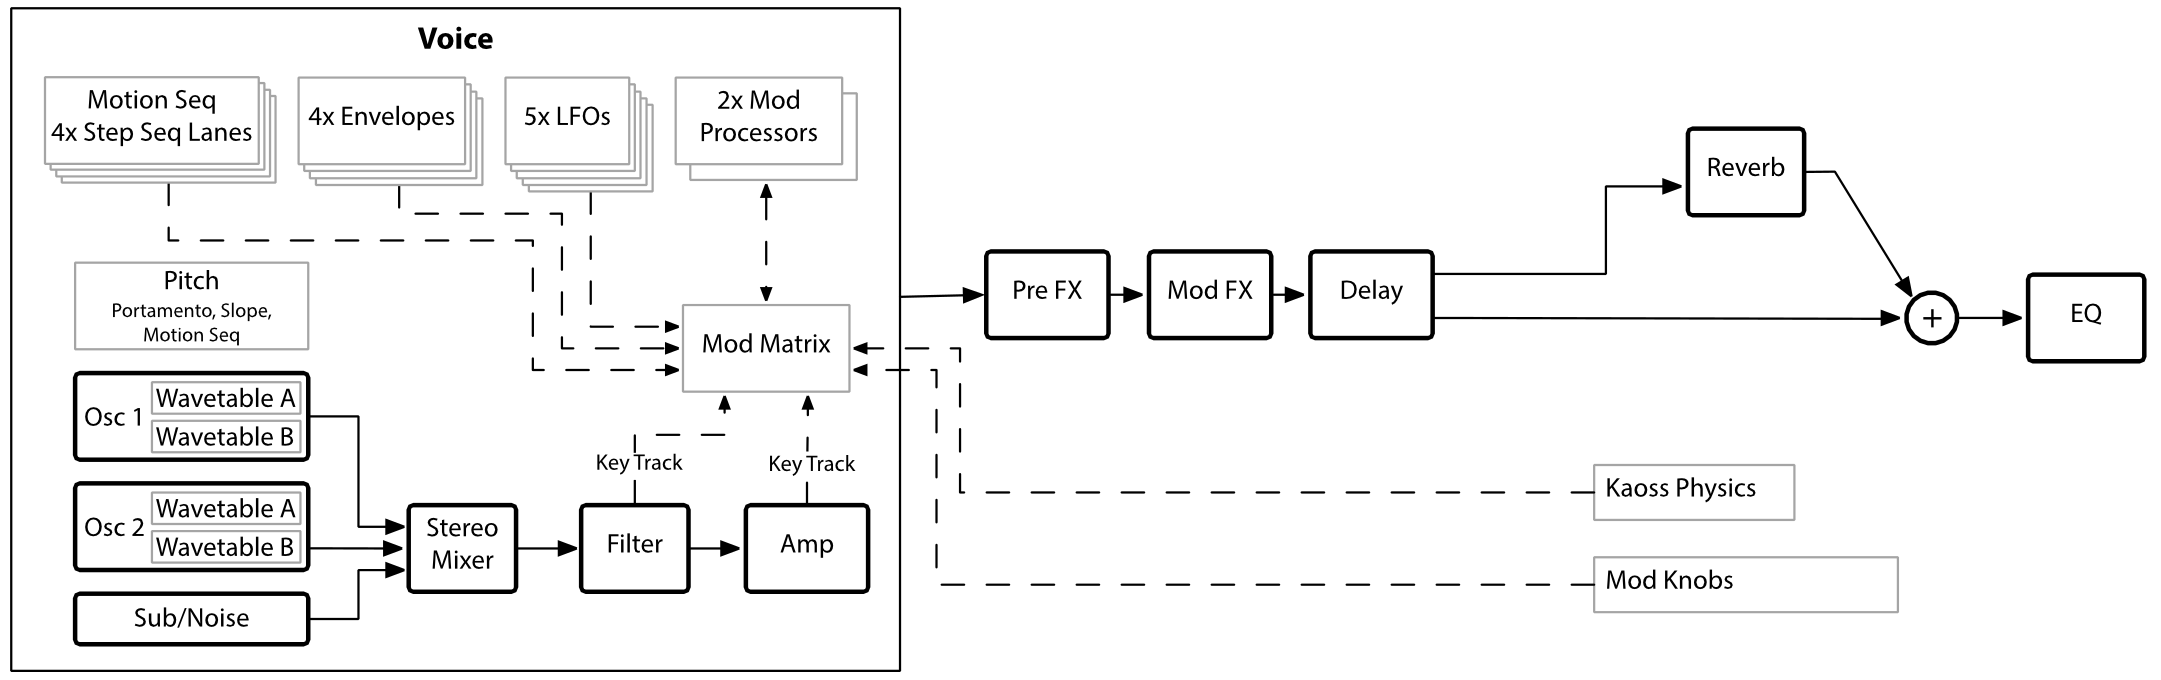
\includegraphics[width=0.9\linewidth]{modwave_diagram.png}

    \caption{
      Diagram blokowy pojedynczego głosu w syntezatorze 
      \textit{Korg Modwave}.
    }
  \end{figure}
\end{frame}





% \begin{frame}
%   \frametitle{Generalizacja tradycyjnego procesu syntezy dźwięku}

%   \begin{enumerate}
%     \item Bloki generujące sygnał:
%       \begin{enumerate}
%         \item synteza prostych sygnałów (sinus, trójkąt, prostokątny),
%         \item odtwarzanie sampli dźwiękowych,
%         \item sygnał modulujący (rytm, \textit{ADSR}).
%       \end{enumerate}
%     \item Bloki przetwarzające sygnał:
%       \begin{enumerate}
%         \item filtry (górnoprzepustowy, dolnoprzepustowy, itd.),
%         \item efekty (pogłos, echo).
%       \end{enumerate}
%     \item Połączenia między blokami:
%       \begin{enumerate}
%         \item modulowanie parametrów generacji/przetwarzania sygnału.
%       \end{enumerate}
%   \end{enumerate}
% \end{frame}

% \begin{frame}
%   \frametitle {Synteza oparta o moduły}

%   \begin{multicols}{2}
%   \begin{figure}
%     \centering
%     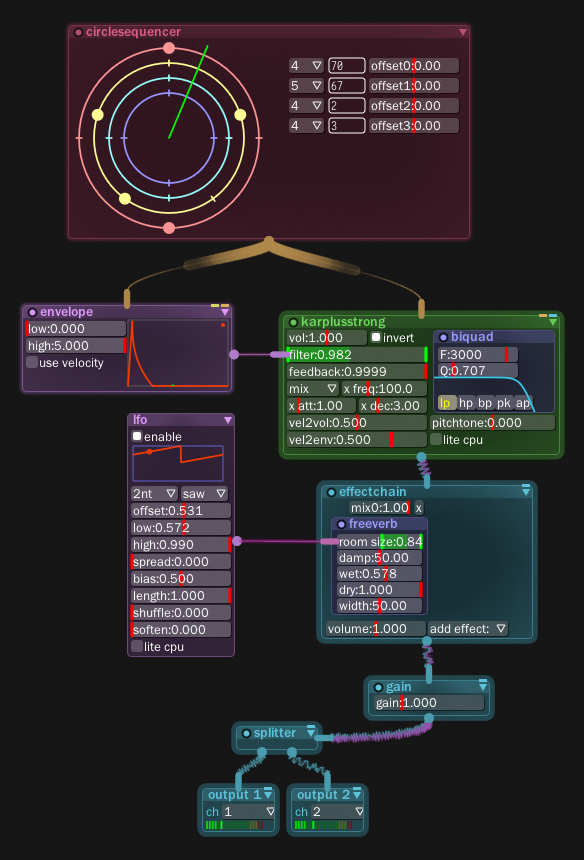
\includegraphics[width=0.6\linewidth]{bespoke.png}
%     \caption{Oprogamowanie \textit{Bespoke}.}
%   \end{figure}

%   \begin{figure}
%     \centering
%     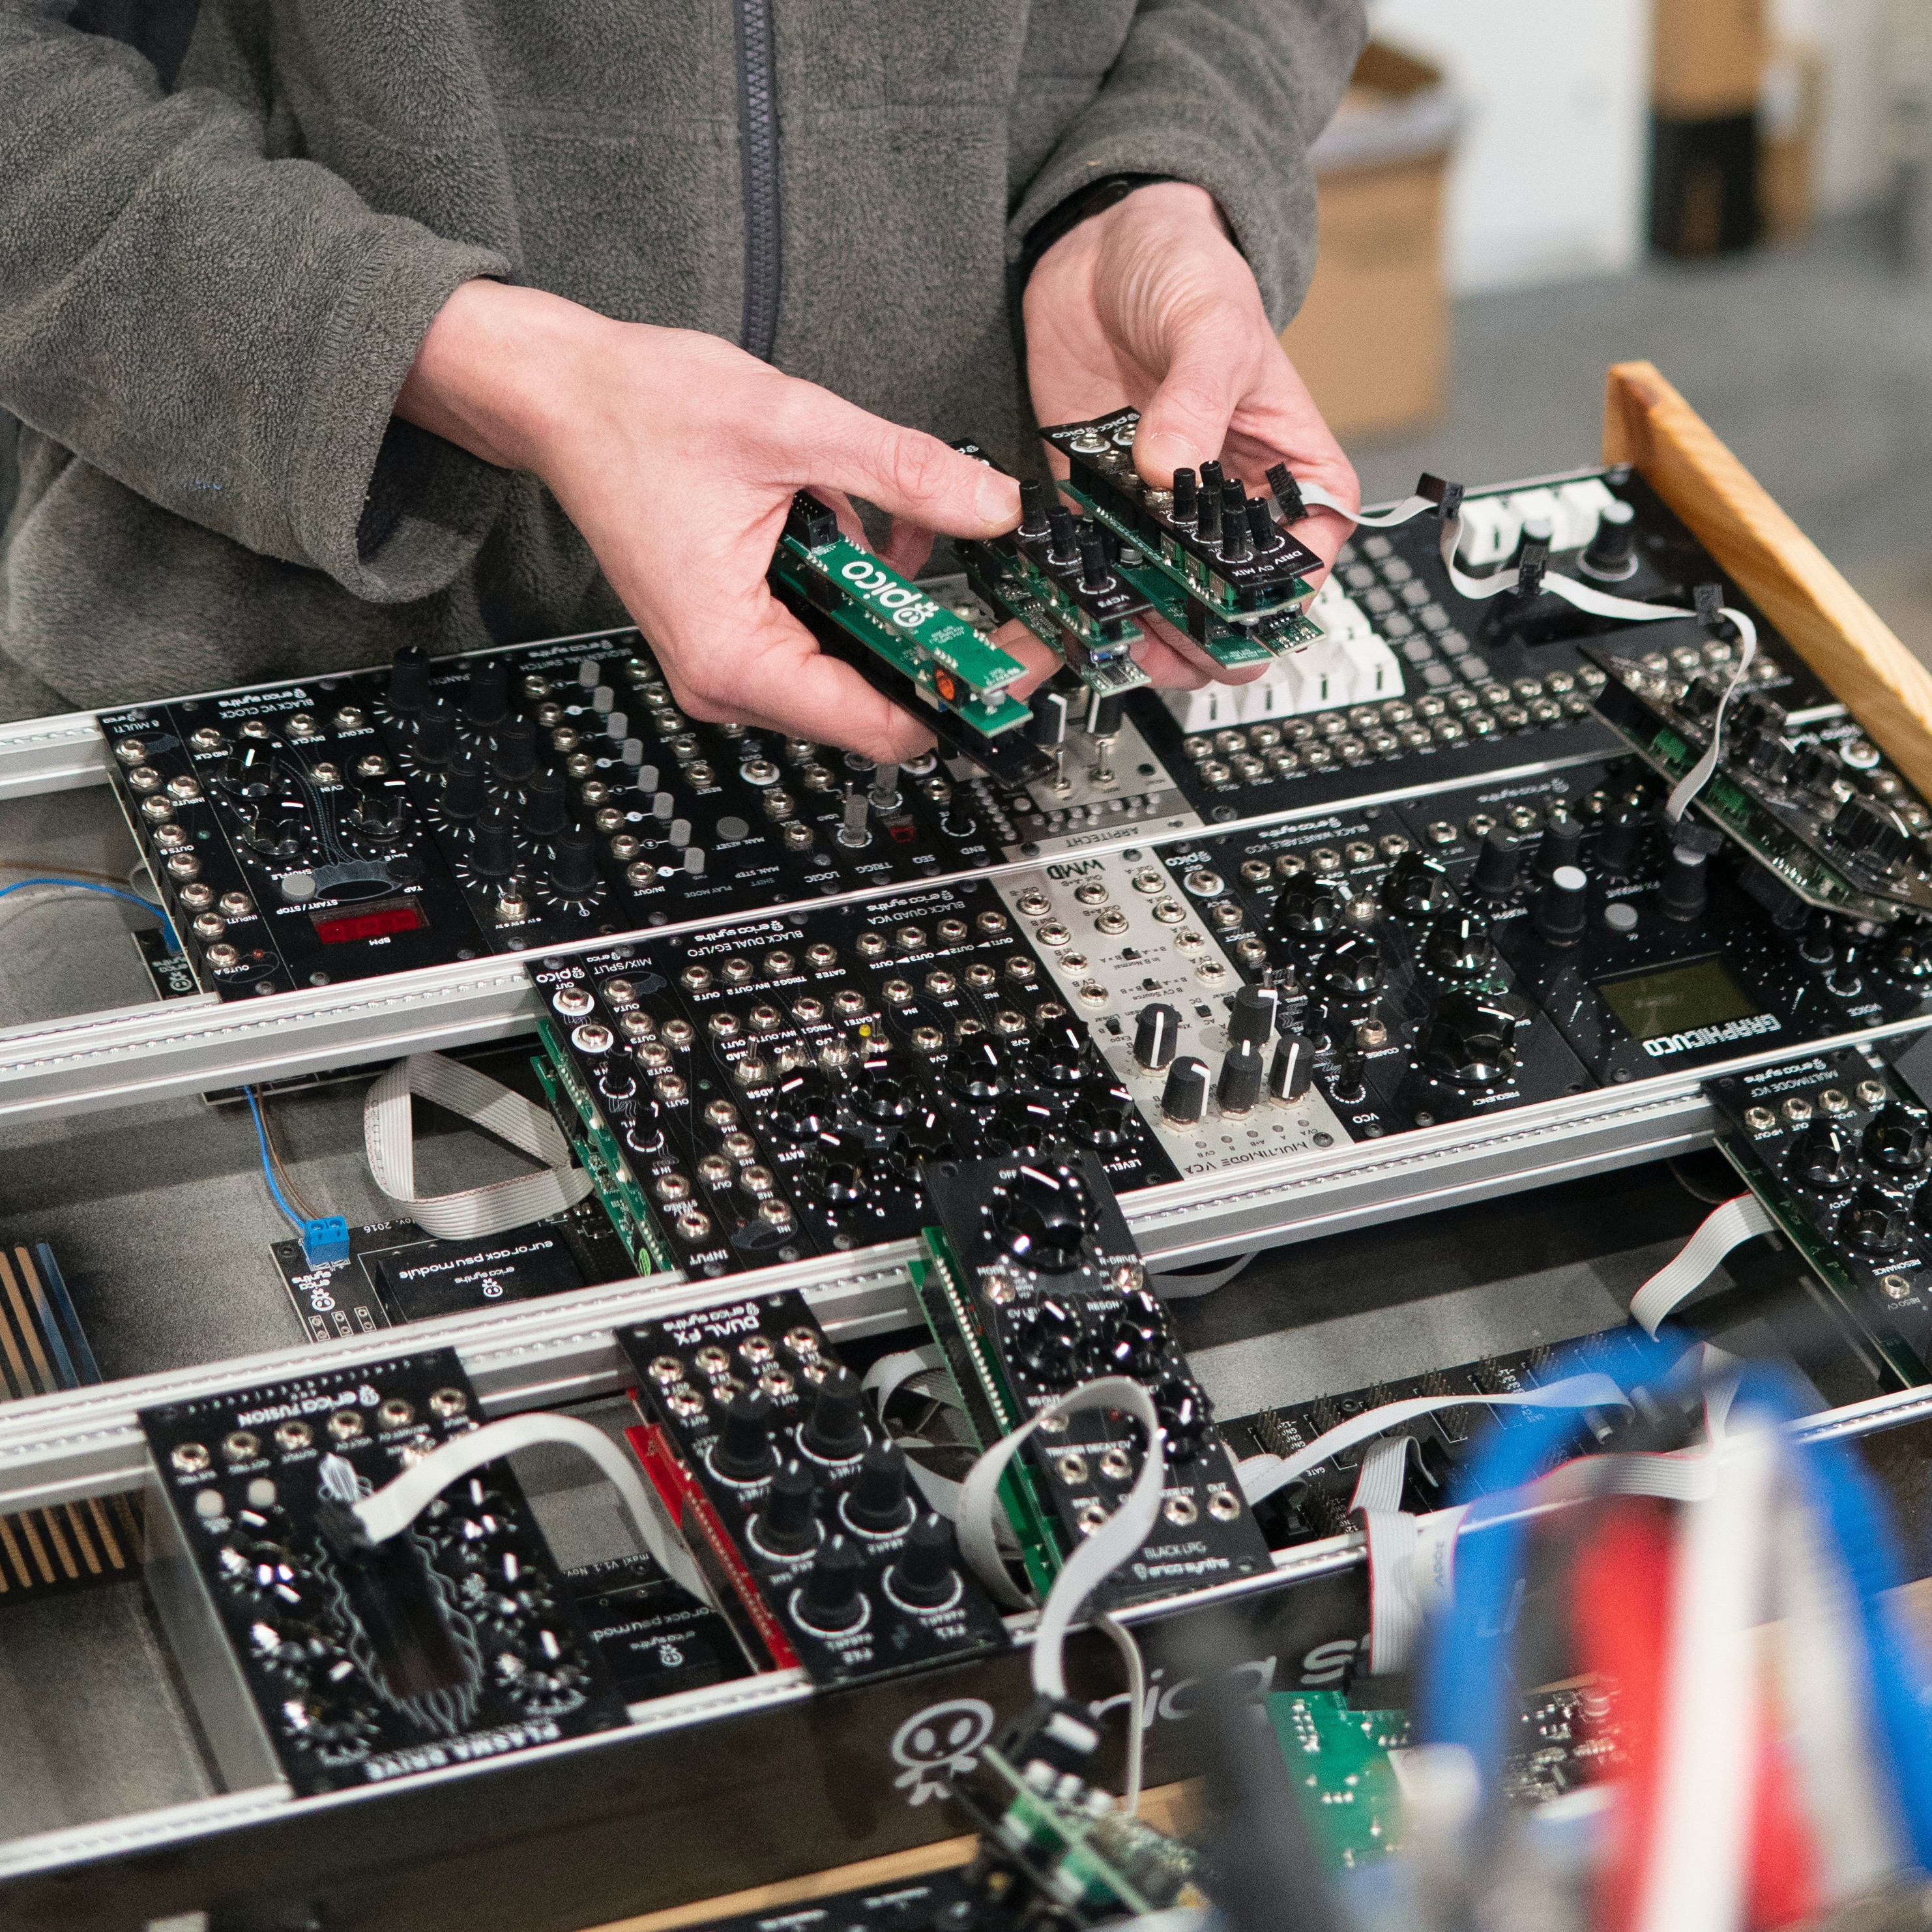
\includegraphics[width=0.9\linewidth]{modular-synth.jpg}
%     \caption{Syntezator modułowy.}
%   \end{figure}
%   \end{multicols}
% \end{frame}

\begin{frame}
  \frametitle{Jak algorytmicznie wyworzyć układ DSP generujący zadany dźwięk?}

  \begin{figure}
    \centering
    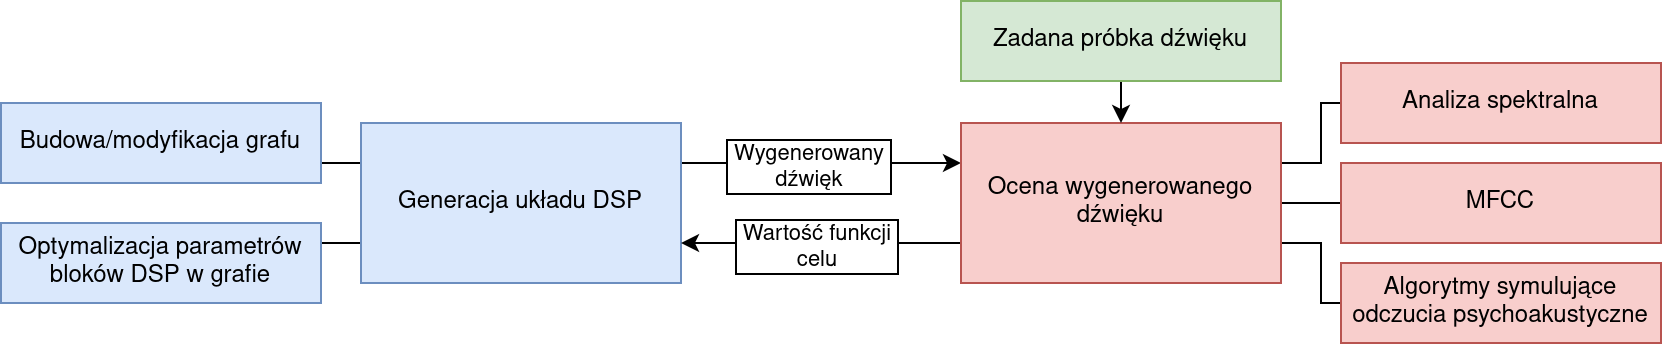
\includegraphics[width=1.0\linewidth]{algorithm-diagram.png}
    \caption{Diagram algorytmu realizowanego w ramach pracy.}
  \end{figure}
\end{frame}


\section{Owoce pracy}
\begin{frame}
  \frametitle{Owoce pracy - silnik syntezy}

  \vspace{-0.5cm}

  \begin{figure}
    \centering
    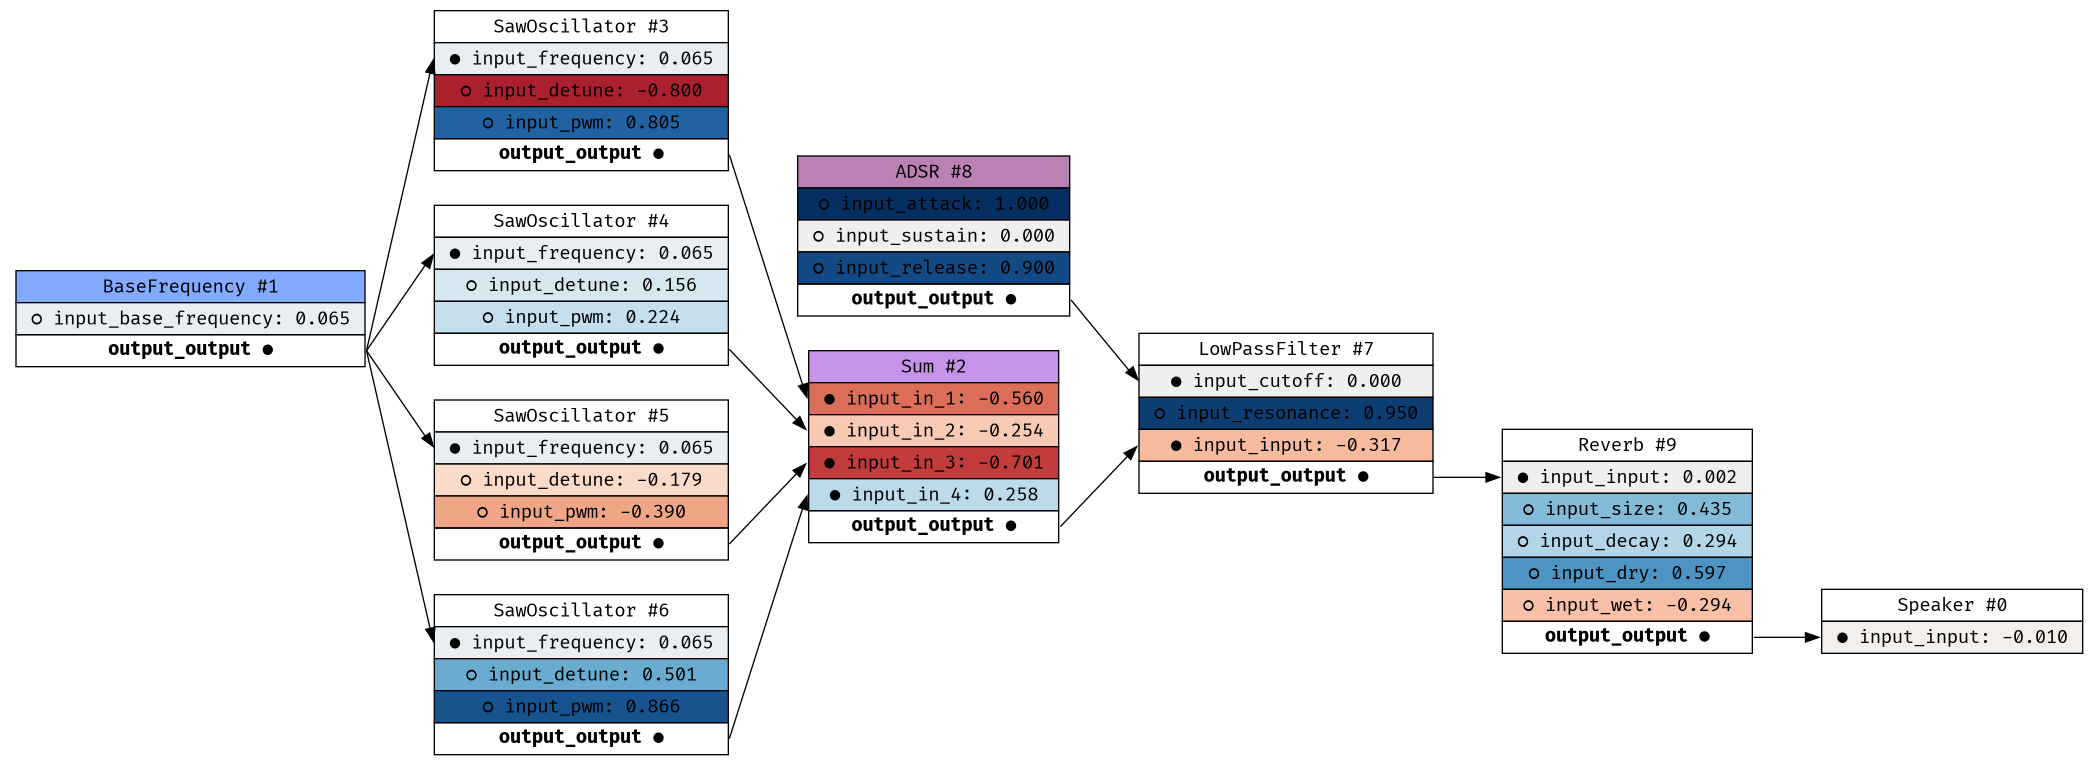
\includegraphics[width=0.8\linewidth]{example_synth.png}
    \caption{Przykładowy graf DSP wygenerowany w środowisku eksperymentowym.}
  \end{figure}

  \vspace{-0.5cm}

  \begin{itemize}
    \item Implementacja w wydajnym, kompilowanym języku \texttt{Rust},
    \item Natywna biblioteka dla języka \texttt{Python},
    \item Generuje struktury danych z pakietu obliczeniowego \texttt{numpy}.
  \end{itemize}
\end{frame}


\begin{frame}
  \frametitle{Owoce pracy - porównanie sygnałów pod względem barwy, czyli funkcja celu}

  \begin{multicols}{2}
  \begin{figure}
    \centering
    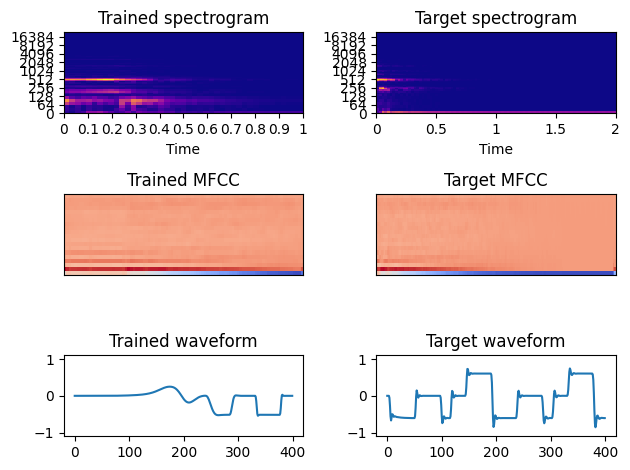
\includegraphics[width=1.0\linewidth]{example_signal_comparison.png}
    \caption{Porównanie sygnałów.}
  \end{figure}

  % co sie tu kurwa dzieje
    \textbf{Wykorzystana funkcja celu: MFCC + DTW}. \\
    \begin{itemize}
      \item \textit{Mel-frequency cepstrum},
      \item \textit{dynamic time warping}.
    \end{itemize}
  
  \end{multicols}
\end{frame}


\section{Ocena stanu pracy}

\begin{frame}
  \frametitle{Osiągnięte cele}

  \begin{enumerate}
    \item Wytworzenie silnika do tworzenia grafów DSP,
    \item Ewolucja parametrów grafu wykonującego syntezę \texttt{FM},
    \item Ewolucja parametrów grafu wykonującego syntezę \texttt{virtual analog},
    \item Ewolucja struktury grafu wykonującego \textit{właściwy} typ syntezy (zależnie od próbki wejściowej).
  \end{enumerate}
\end{frame}


% \begin{frame}
%   \frametitle{Dalszy harmonogram realizacji pracy}

%   \begin{enumerate}
%     \item \textbf{Cel został osiągnięty}: opracowany algorytm generuje grafy DSP, które upodobniają się do zadanych próbek dźwięku:
%       \begin{itemize}
%         \item Wciąż możliwe jest poprawienie dokładności,
%         \item Wciąż możliwe jest przyspieszenie czasu trenowania,
%         \item Wciąż można implementować nowe bloki DSP,
%       \end{itemize}
%     \item Postęp w pisaniu pracy: $\sim$15\%.
%   \end{enumerate}
% \end{frame}

\begin{frame}
  \frametitle{Potencjalne kierunki dalszego rozwoju}

  \begin{enumerate}
    \item Przetestowanie alternatywnych struktur genotypu reprezentującego strukturę grafu,
    \item Implementacja funkcji celu na \texttt{GPU}~\cite{gpu_fft},
    \item Inkrementalne trenowanie na coraz dłuższych fragmentach docelowej próbki,
  \end{enumerate}
\end{frame}



\section{Bibliografia}

\begin{frame}
  \begin{thebibliography}{99} % Beamer does not support BibTeX so references must be nserted manually as below

  \bibitem[Zhang, 2023]{language_models_drummers} Zhang, Li and Callison-Burch, Chris
  \newblock Language Models are Drummers: Drum Composition with Natural Language Pre-Training
  \newblock \url{https://arxiv.org/abs/2301.01162}

  \bibitem[Forsgren, 2023]{riffusion} Forsgren, Seth* and Martiros, Hayk*
  \newblock Riffusion - Stable diffusion for real-time music generation
  \newblock \url{https://riffusion.com/about},

  \bibitem[Engel, 2017]{nsynth} Jesse and Resnick, Cinjon and Roberts, Adam and Dieleman, Sander and Eck, Douglas and Simonyan, Karen and Norouzi, Mohammad
  \newblock Neural Audio Synthesis of Musical Notes with WaveNet Autoencoders
  \newblock \url{https://arxiv.org/abs/1704.01279}

  \end{thebibliography}
\end{frame}

\begin{frame}
  \begin{thebibliography}{99} % Beamer does not support BibTeX so references must be nserted manually as below
  \bibitem[Faronbi, 2023]{multi_task_synth_programming} Faronbi, Daniel and Roman, Iran and Bello, Juan Pablo,
  \newblock Exploring Approaches to Multi-Task Automatic Synthesizer Programming
  \newblock \url{10.1109/ICASSP49357.2023.10095540}

  \bibitem[Yan]{music_identification} Yan Ke and Hoiem, D. and Sukthankar, R.
  \newblock Computer vision for music identification
  \newblock \texttt{10.1109/CVPR.2005.105}

  \bibitem[Macret]{puredata} M. & Pasquier, P.
  \newblock Automatic Design of Sound Synthesizers as Pure Data Patches using Coevolutionary Mixed-typed Cartesian Genetic Programming
  \newblock \url{https://metacreation.net/wp-content/uploads/2015/08/p309-macret.pdf}

  \end{thebibliography}
\end{frame}

\begin{frame}
  \begin{thebibliography}{99} % Beamer does not support BibTeX so references must be nserted manually as below

    \bibitem[Caspe]{ddx7} Caspe, Franco and McPherson, Andrew and Sandler, Mark
    \newblock DDX7: Differentiable FM Synthesis of Musical Instrument Sounds
    \newblock \url{https://arxiv.org/abs/2208.06169}

    \bibitem[Jacobsen]{sliding_fourier} Jacobsen, E. and Lyons, R.
    \newblock The Sliding Fourier
    \newblock \texttt{10.1109/MSP.2003.1184347}

    \bibitem[Nvidia]{gpu_fft} NVIDIA Corporation & Affiliates.
    \newblock NVIDIA® CUDA® Fast Fourier Transform (FFT)
    \newblock \url{https://docs.nvidia.com/cuda/cufft/index.html}

  \end{thebibliography}
\end{frame}

\begin{frame}
  % \frametitle{Cel pracy}

  % \vspace{-0.5cm}
  % \begin{figure}
  %   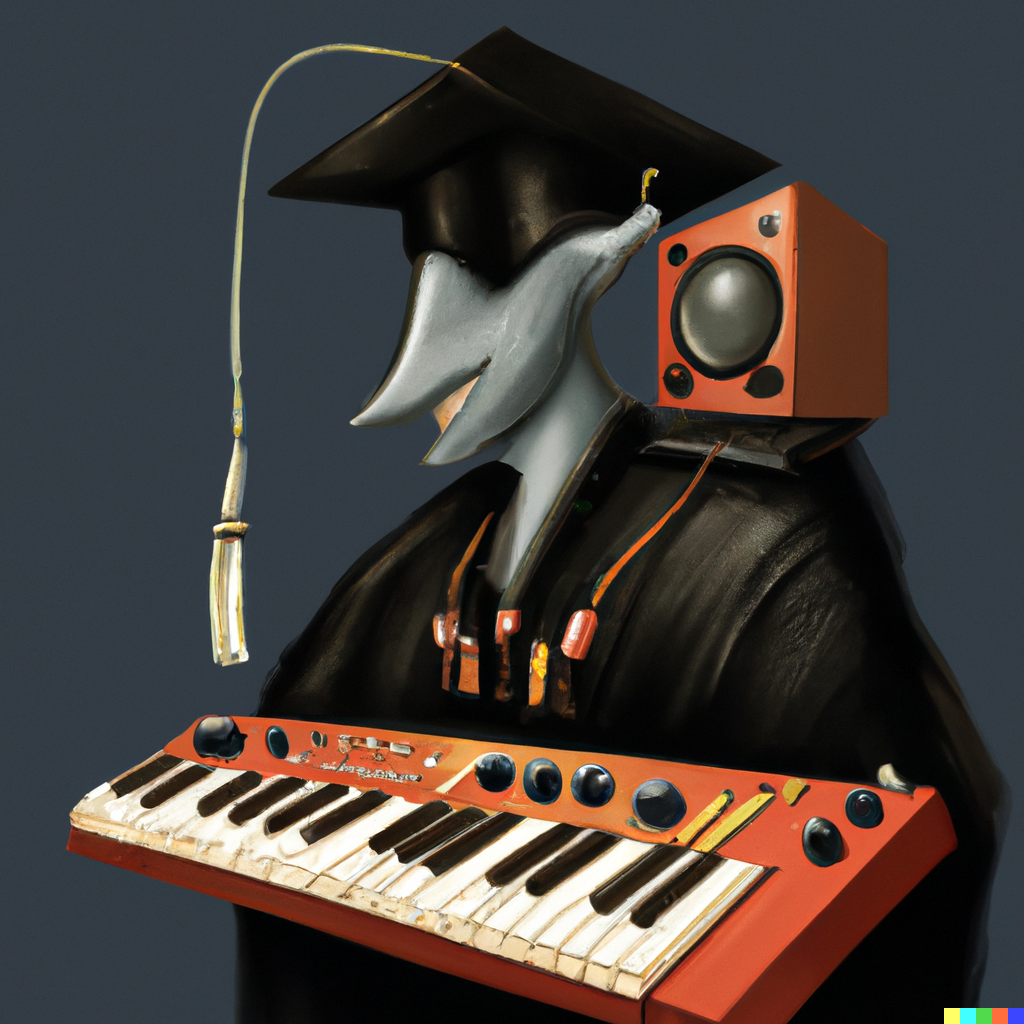
\includegraphics[width=0.4\linewidth]{./synth_graduating_from_uni.png}
  %   \caption{Obraz wygenerowany przez \texttt{DALL-E} dla promptu ,,\textit{sound synthesizer graduating from university}''.}
  % \end{figure}

  \centering
  \Large
  Dziękuję za uwagę!
    % \colorbox{blue}{\color{white}\textbf{Dziękuję za uwagę!}}
    % Wytworzenie grafu przetwarzania sygnałów, generującego dźwięk o określonej 
\end{frame}

% \begin{frame}
%   \frametitle{Deklaracja}

%   % \vspace{-0.5cm}
%   % \begin{figure}
%   %   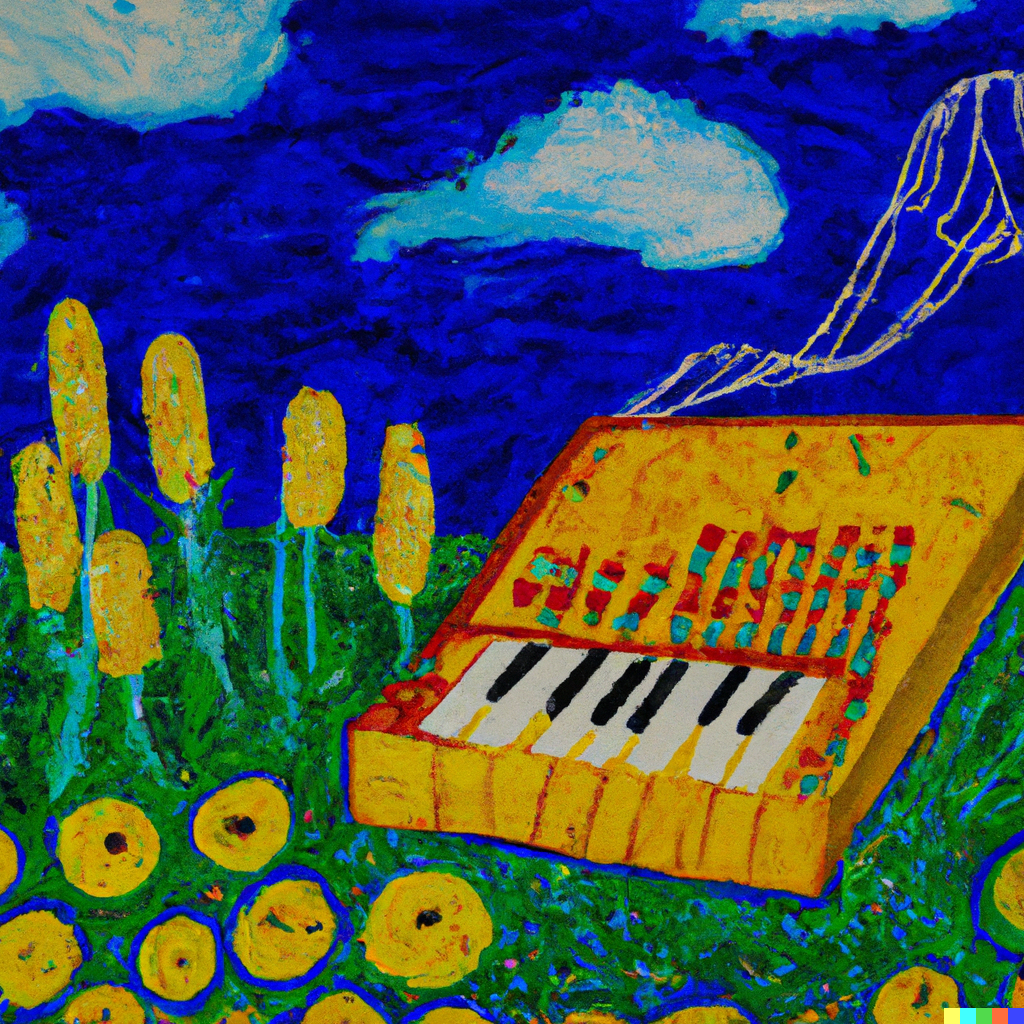
\includegraphics[width=0.4\linewidth]{van_gogh_synth.png}
%   %   \caption{Obraz wygenerowany przez \texttt{DALL-E} dla promptu ,,\textit{sound synthesizer drawn in in style of van Gogh}''.}
%   % \end{figure}
%   {
%   \Large
%   Deklaruję, iż uda się ukończyć pracę przed wyznaczonym terminem obrony.
%   }

%   $\sim$ Mateusz Bączek
%     % \colorbox{blue}{\color{white}\textbf{Dziękuję za uwagę!}}
%     % Wytworzenie grafu przetwarzania sygnałów, generującego dźwięk o określonej 
% \end{frame}

\end{document}

